\chapter{Use Cases}

\section{Introduction}
This section describes the four to five main use cases that an actor can perform. The first subsection contains a diagram displaying the main user and the user's four to five possible actions. The second subsection details the name, goal, conditions, and steps corresponding to each use case. 

\section{Diagrams}
\begin{figure}[!ht]
      \centering
      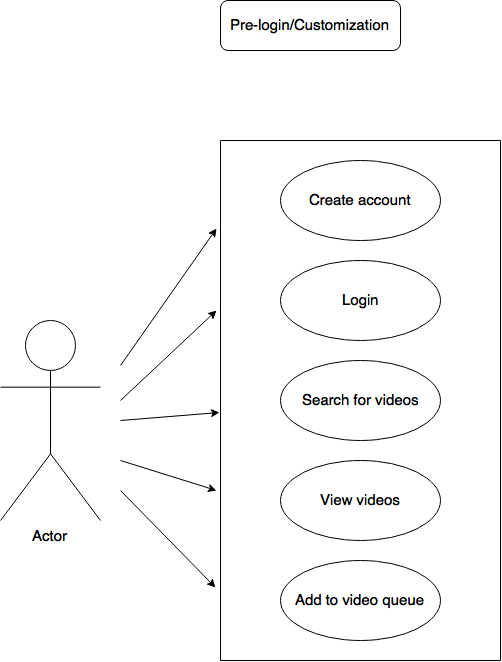
\includegraphics[width=0.5\textwidth]{useCasePreLogin}
      \caption{Use Case Diagram of Pre-login}	
\end{figure}
\begin{figure}[!ht]
      \centering
      \includegraphics[width=0.5\textwidth]{useCasePostLogin}
      \caption{Use Case Diagram of Post-login}	
\end{figure}


\section{Use Case Description}
\begin{itemize}
\item Create account
	\begin{itemize}
	\item Name: Create an account to be used on website
    \item Goal: To create an account to be used on website
    \item Actor: User
    \item Preconditions
		\begin{enumerate}
		\item User must be on webpage
        \end{enumerate}
    \item Steps
    	\begin{enumerate}
		\item User selects my settings
        \item User enters desired username and password combination
        \item User submits username and login combination to system to be submitted
        \end{enumerate}
    \item Post-conditions
		\begin{enumerate}
		\item Assuming user's username is unique, the combination gets saved to the system
        \item The website grabs user's stored data and allows for user customization 
        \item The website returns to the overall view of the website with user now logged-in
        \item The website loads personalized customization settings
        \end{enumerate}
    \item Exceptions
    	\begin{enumerate} 
    	\item User's username needs to be unique so process may need to be repeated to achieve a unique result, user will be alerted of error occurring 
        \end{enumerate}
    \end{itemize}

\item Login
	\begin{itemize}
	\item Name: Login to website
    \item Goal: To sign in to website
    \item Actor: User
    \item Preconditions
		\begin{enumerate}
		\item User must be on webpage
        \item User must have a preexisting account
        \end{enumerate}
    \item Steps
    	\begin{enumerate}
		\item User selects my settings
        \item User enters login credentials
        \item User submits login to be signed into website
        \end{enumerate}
    \item Post-conditions
		\begin{enumerate}
		\item User's username is checked if it exists in the system
        \item The matching username and password are returned 
        \item The user's password is then checked against the returned username's password
        \item Assuming the credentials match, the user is then logged on to the system
        \end{enumerate}
    \item Exceptions
    	\begin{enumerate} 
    	\item User who has entered information but has not created an account will be alerted that their information was not found in the system
        \end{enumerate}
    \end{itemize}
    
\item Search for Videos
	\begin{itemize}
	\item Name: Search for videos 
    \item Goal: Allows user to specify videos to watch
    \item Actor: User
    \item Preconditions
		\begin{enumerate}
		\item User must be on webpage
        \end{enumerate}
    \item Steps
    	\begin{enumerate}
		\item User types into textbox to specify which sports video to view
        \item User views the returned results from his query
        \end{enumerate}
    \item Post-conditions
    	\begin{enumerate}
		\item User continues on website to add videos to queue
        \end{enumerate}
    \item Exceptions
    	\begin{enumerate}
        \item Video requested by the user may be unavailable in database of video sources, so user can modify search items to perform another search
    	\end{enumerate}
    \end{itemize}

\item View Videos
	\begin{itemize}
	\item Name: View videos 
    \item Goal: To watch video on website
    \item Actor: User
    \item Preconditions
		\begin{enumerate}
		\item User must be on webpage
        \item User must allow video to play
        \end{enumerate}
    \item Steps
    	\begin{enumerate}
		\item User able to enjoy video playback
        \end{enumerate}
    \item Post-conditions N/a
    \item Exceptions N/A
    \end{itemize}
    
\item Add to Video Queue
	\begin{itemize}
	\item Name: Add videos to queue
    \item Goal: To use website to add user specific videos to queue
    \item Actor: User
    \item Preconditions
		\begin{enumerate}
		\item User must be on webpage
        \item User must have already searched for video(s)
        \end{enumerate}
    \item Steps
    	\begin{enumerate}
		\item User clicks on desired video(s) from search results
        \item Video is added to the front of the queue
        \item Video is ready to be viewed in order displayed by queue
        \end{enumerate}
    \item Post-conditions
    	\begin{enumerate}
		\item To view video user must allow current video to play through
        \end{enumerate}
    \item Exceptions
    	\begin{enumerate}
    	\item If the user has had added their desired video to the queue after the current video has finished playing then it will be queued up as the next video to be played
    	\end{enumerate}
    \end{itemize}
    
\item Customize Settings
	\begin{itemize}
	\item Name: Customize settings
    \item Goal: To customize personal settings
    \item Actor: User
    \item Preconditions
		\begin{enumerate}
		\item User must be on webpage
        \item User must have an account and be logged into system
        \end{enumerate}
    \item Steps
    	\begin{enumerate}
        \item User can edit their personalization choices for their favorite teams
        \end{enumerate}
    \item Post-conditions
    	\begin{enumerate}
		\item User must save changes made when editing their profile by selecting to return to go home
        \end{enumerate}
    \item Exceptions
    	\item User quits web browser before properly navigating to the home screen to save updated preferences
    \end{itemize}
    
\item View Customized Videos
	\begin{itemize}
	\item Name: View customized videos 
    \item Goal: To view list of customized videos
    \item Actor: User
    \item Preconditions
		\begin{enumerate}
		\item User must be on webpage
        \item User must be logged into system
       	\item User must have edited and saved their preferences
        \end{enumerate}
    \item Steps
    	\begin{enumerate}
		\item User returns back to home page of website
        \item User can select personalized video selection displayed in the search result column 
        \end{enumerate}
    \item Post-conditions
    	\begin{enumerate}
		\item The program grabs the desired personalized entries
        \item Videos will play in most recent found from database
        \end{enumerate}
    \item Exceptions
    	\begin{enumerate}
    	\item The customized results returned may return previously watched videos as the system grabs the most recent videos added to the database
    	\end{enumerate}
    \end{itemize}
    
\item Sign Out
	\begin{itemize}
	\item Name: Sign out of website
    \item Goal: To sign out the users profile from the website
    \item Actor: User
    \item Preconditions
		\begin{enumerate}
		\item User must be on webpage
        \item User must be signed in to the system
        \end{enumerate}
    \item Steps
    	\begin{enumerate}
		\item User clicks sign off button
        \item User profile exits the system
        \end{enumerate}
    \item Post-conditions
    	\begin{enumerate}
		\item Clear user personalized data from the website
        \item Reset the website so it functions as if a new user has just entered 
        \end{enumerate}
    \item Exceptions N/A
    \end{itemize}
    
\end{itemize}